% Appendix Template

\chapter{Examples implementing ETPs} % Main appendix title

\label{AppendixETPexample} % Change X to a consecutive letter; for referencing this appendix elsewhere, use \ref{AppendixX}

The following sections contain examples of clinical trials that have implemented Efficacy Transition Pathways (ETPs). All of these trials were designed by statisticians at the Cancer Research UK Clinical Trials Unit (CRCTU) at the University of Birmingham.

%-----------------------------------
%	SUBSECTION 1
%-----------------------------------

\section{MonoGerm} 

This trial was designed by Lucinda Billingham (LB) and Laura Kirton (LK). What is presented here is the design that was used as part of a grant application which has since been accepted. The trial is currently in the process of being set-up so may be subject to some design changes before it is open. 

MonoGerm \footnote{A phase II trial of carboplatin or vinblastine monotherapy induction prior to radiotherapy for patients with intracranial germinoma} is a Phase \RN{2} trial investigating, in parallel, two single-agent chemotherapies (carboplatin or vinblastine) as monotherapy prior to standard of care radiotherapy in patients with intracranial germinoma. This trial utilises a Bayesian approach for analysis and decision making. A 'flip-flop' approach is used for recruitment \cite{harringtonGuidelinesPreclinicalEarly2011}. Essentially, recruitment will begin to the carboplatin arm then once three patients have been recruited and considered evaluable for an interim analysis recruitment flips to the vinblastine arm. This process is then repeated by switching recruitment back and forth between the two arms till recruitment is complete. 

Typically intracranial germinoma is chemosensitive but it requires radiotherapy for a cure. This mainly affects a paediatric population. For patients with localised disease, standard of care involves three-drug chemotherapy consisting of ifosfamide, carboplatin and etoposide followed by subsequent radiotherapy. Treatment involving multiple chemotherapies allows for reduction in radiotherapy doses and fields. However, there is still an increased burden of treatment on patients which can cause both short and long-term harm. This can lead to patients experiencing multiple toxicities such as diabetes insipidus, myelosuppression, vomiting/diarrhoea, electrolyte disturbances, renal impairment, and elevation of liver enzymes. 

The aim of the trial is to evaluate whether a single-agent chemotherapy (carboplatin or vinblastine) is non-inferior to	the standard of care multi-drug chemotherapy for inducing complete response (CR), and is associated with reduced harm and improved quality of life. The primary outcome measure will be CR based on MRI scans at 6 and 12 weeks. 

The trial will consist of two arms, one arm for carboplatin and one for vinblastine. There will be 36 patients recruited in total, 18 per arm. Patients will be enrolled in cohorts of three to each treatment-arm by the flip-flop design. This is illustrated in Figure \ref{fig_etp:MonoGermFlipFlop}. Recruitment begins in the carboplatin arm and then once three patients have been recruited recruitment is paused and then begins in the vinblastine arm. Whilst recruitment is paused in the carboplatin arm an interim analysis will be performed for that first cohort. Here primary outcome data and key safety data will be assessed. Once recruitment to the first cohort of the vinblastine arm is complete and the interim analysis for the first cohort of carboplatin patients is done, recruitment can begin for the second cohort in the carboplatin arm and the interim analysis for the first cohort of vinblastine patients can be conducted. This process is then repeated for the subsequent cohorts. This design allows for continuous enrolment and monitoring of the primary outcome. 

\begin{figure}[h!]
	\centering
	\caption{Flip-flop recruitment design in the MonoGerm trial.}
	\label{fig_etp:MonoGermFlipFlop}
	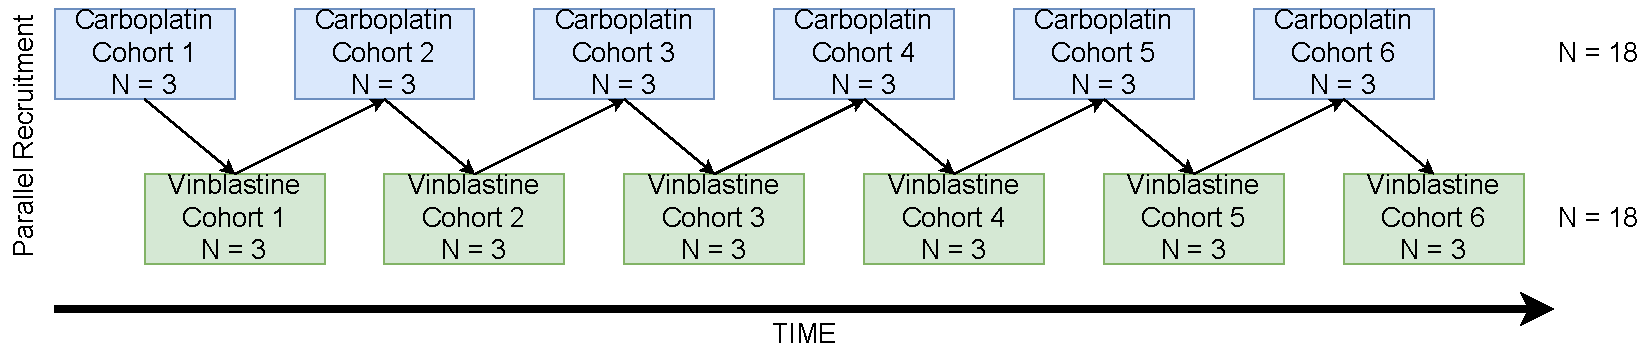
\includegraphics[width=\textwidth]{ETP-MonoGermFlipFlop}
\end{figure}

A Bayesian approach is implemented to assess the true CR rates. Specifically, the experimental monotherapies will need to demonstrate non-inferiority to the standard of care by a clinically acceptable margin. Based on previous data it was determined that the minimum CR rate with standard of care is 30\%. This value was taken as the non-inferiority margin. So, if the treatments have a CR rate $\geq30$\% they will be considered non-inferior. 

CR rates for each treatment arm will be established from the posterior probability distribution generated using a beta-binomial conjugate analysis. A minimally informative Beta(1,1) prior will be used in combination with the data observed during the trial to produce the posterior. In terms of decision making the following rule for the final analysis was specified: 

\begin{equation}
	P(CR \geq 30\%) \geq 0.8
\end{equation}

That is to say that if there is a high probability ($\geq 0.8$) that the true CR rate is $\geq30$\% there will be a GO decision, which in the context of this trial means the treatment arm would be deemed non-inferior. The minimum number of observed CRs out of the 18 patients needed to warrant a GO decision is seven. If seven responses are observed the median Bayesian estimate of the CR rate would be 40\% with a 0.82 probability that the true CR rate is $\geq30$\%. 

Stopping rules have also been implemented. At each interim analysis the predicted probability of success (PPoS) will be calculated. This is the probability that a GO decision would be made at the final analysis based on current data that has been accrued. Here the stopping rule is such that if the PPoS is less than 0.01 we would recommend stopping recruitment to that arm. 

It is important to note that whilst the trial has two arms it is not designed with the intention of making comparisons between the two treatments. Rather the trial aims to find if there is enough evidence that one of these treatments provides a sufficient response rate to warrant a GO decision.  

LK produced ETPs throughout the design of this trial. Figure \ref{fig_etp:MonoGermETP} shows the ETP for the design specified here. The ETPs produced here helped determine what data we wanted to present as well as how we structure the data in each of the cells. Here each cell shows the number of responses, the PPoS or the posterior probability that the response rate is $\geq30$\%, the Bayesian estimate of CR rate and a lower one-sided 80\% credible interval.

Calculations for these plots were conducted in STATA and the ETP was produced in Microsoft PowerPoint. One benefit of this approach is that the ETP can be easily customised and labelled. However, this meant that any changes in the design that affected the decision-making resulted in the ETP having to be updated manually. As a tool the ETP is effective at illustrating a final design but without the ability to easily generate them during the design of a trial they somewhat lose their purpose. This served as further motivation to produce some code or a tool that would allow for ETPs to be automatically created. 

\begin{sidewaysfigure}[h!]
	\centering
	\caption{ETP for the MonoGerm trial.}
	\label{fig_etp:MonoGermETP}
	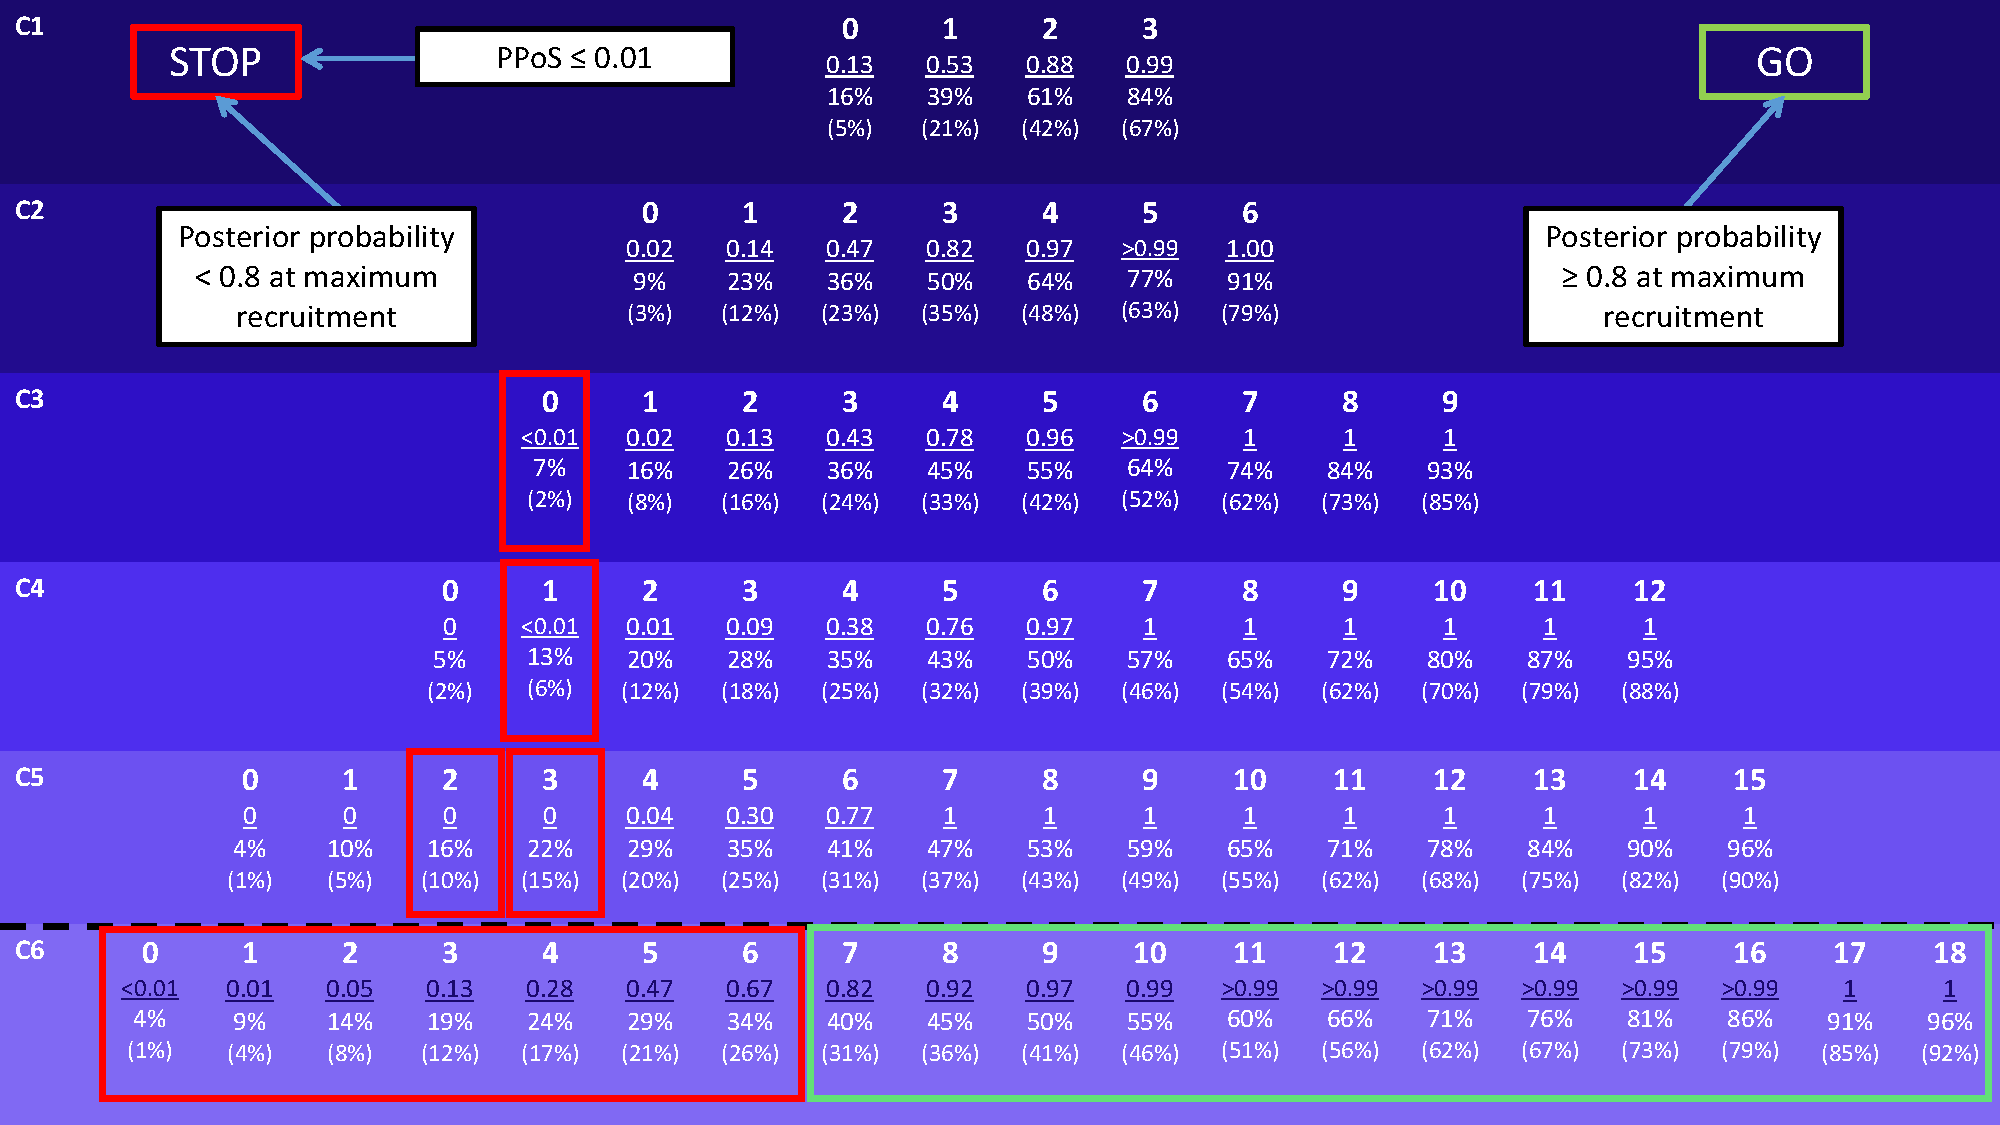
\includegraphics[width=23cm, height=15cm]{ETP-MonoGermETP}
\end{sidewaysfigure} 

\clearpage

%-----------------------------------
%	SUBSECTION 2
%-----------------------------------

\section{Glo-BNHL}

This trial was designed by Lucinda Billingham (LB) with the assistance of Shanna Maycock (SM). During initial stages of the design Grace Holt (GH) also assisted with the implementation of ETPs. This trial is currently still in set-up so specific details of the trial may be subject to change.   

The Glo-BNHL \footnote{A Global Study of Novel Agents in Paediatric and Adolescent Relapsed and Refractory B-cell Non-Hodgkin Lymphoma} study is a platform trial that aims to investigate the safety and effectiveness of novel treatments in children, adolescents and young adults with relapsed and/or refractory B-cell non-Hodgkin Lymphoma (r/r BNHL). This trial is an international collaboration and hopes to generate substantial evidence that could change practice in this rare cancer population. 

Inclusion of novel agents into the platform will be determined by an international Trial Steering Committee (TSC). Currently the platform consists of three separate treatment arms, each focusing on a different novel agent in a distinct group of patients. Each treatment arm will be treated independently which allows for them to be analysed separately. There may also be separate eligibility criteria for each arm. Patients will be enrolled into any arm where they are eligible. The three arms that will be available at the start of the trial are as follows: 

\begin{itemize}
	\item Treatment Arm \RN{1}: Bispecific Antibody (BsAb)
	\item Treatment Arm \RN{2}: Antibody-Drug Conjugate (ADC) with standard \\ chemotherapy
	\item Treatment Arm \RN{3}: Chimeric Antigen Receptor (CAR) T-cells
\end{itemize}

This trial utilises an adaptive Bayesian design, which enables GO/No GO decisions specific to the distinct populations in each treatment arm. The Bayesian approach has many benefits here as it facilitates decision making with small sample sizes. Decisions will be made based on the estimate of the probability that a novel agent is clinically effective. The specific criteria will vary between each treatment arm. This design and approach also allows for continuous evaluation of each novel agent. Treatment arms may be removed if the treatment is shown to be ineffective based on the trial data. Additionally, treatment arms may also be added or amended in the future if recommended by the TSC. 

Treatment arm \RN{1} aims to estimate the clinical efficacy of BsAb treatment in patients with r/r BNHL in first (only one prior line of therapy) or subsequent relapse (more than one prior line of therapy). Due to this treatment arm \RN{1} is split into two groups, \RN{1}a and \RN{1}b for patients with one relapse or more than one relapse respectively. These two subsequent arms will be recruited into and analysed separately. In terms of treatment these patients will receive odronextamab given as an intravenous infusion weekly for 12 weeks, then every two weeks until nine months, and every four weeks thereafter until progression or for a maximum of two years. The outcome measure for patients in treatment arms \RN{1}a and \RN{1}b is the occurrence of an objective response (OR) i.e. complete response (CR) or partial response (PR) after 12 weeks of treatment assessed by Independent Central Review. However, for interim analyses local response assessments will be used. 

Treatment arm \RN{2} aims to estimate the clinical efficacy of ADC treatment with modified R-ICE (rituximab, ifosphamide, carboplatin, etoposide and dexamethasone) chemotherapy in patients with r/r B-NHL in first or subsequent relapse. Patients will receive loncastuximab tesirine given as a 30 minute intravenous infusion with each cycle of modified R-ICE for a maximum of three cycles. Here the outcome measure is occurrence of CR within a maximum of three cycles of treatment. 

Treatment arm \RN{3} aims to estimate the efficacy of CAR T-cell therapy in r/r B-NHL patients who have CAR T-cell product available. The specific treatments patients will receive is yet to be defined. The outcome measure is the occurrence of OR following CAR T-cell infusion. 

Each treatment arm and subsequent treatment arm (i.e. \RN{1}a and \RN{1}b) will aim to recruit 15 evaluable patients during the initial stage. Once this recruitment is complete a transition analysis is performed leading to three possible outcomes. If the analysis results in a No GO decision recruitment to that treatment arm will stop. If the analysis result is a GO decision there are two options either there is sufficient evidence to change practice so the trial will stop recruiting or this will trigger an expansion stage in which a further 15 patients will be recruited. Following the expansion stage a confirmatory analysis will be conducted on all 30 evaluable patients. 

Interim analyses will be conducted after every three patients during the initial stage and after every five patients during the expansion stage. There will also be the option to stop recruitment to a treatment arm based on the data observed in the interim analysis. Figure \ref{fig_etp:Glo-BNHLflowchart} shows a flowchart of the decision making process for each arm in the trial. 

\begin{figure}[h!]
	\centering
	\caption{Flowchart of the decision making process in Glo-BNHL.}
	\label{fig_etp:Glo-BNHLflowchart}
	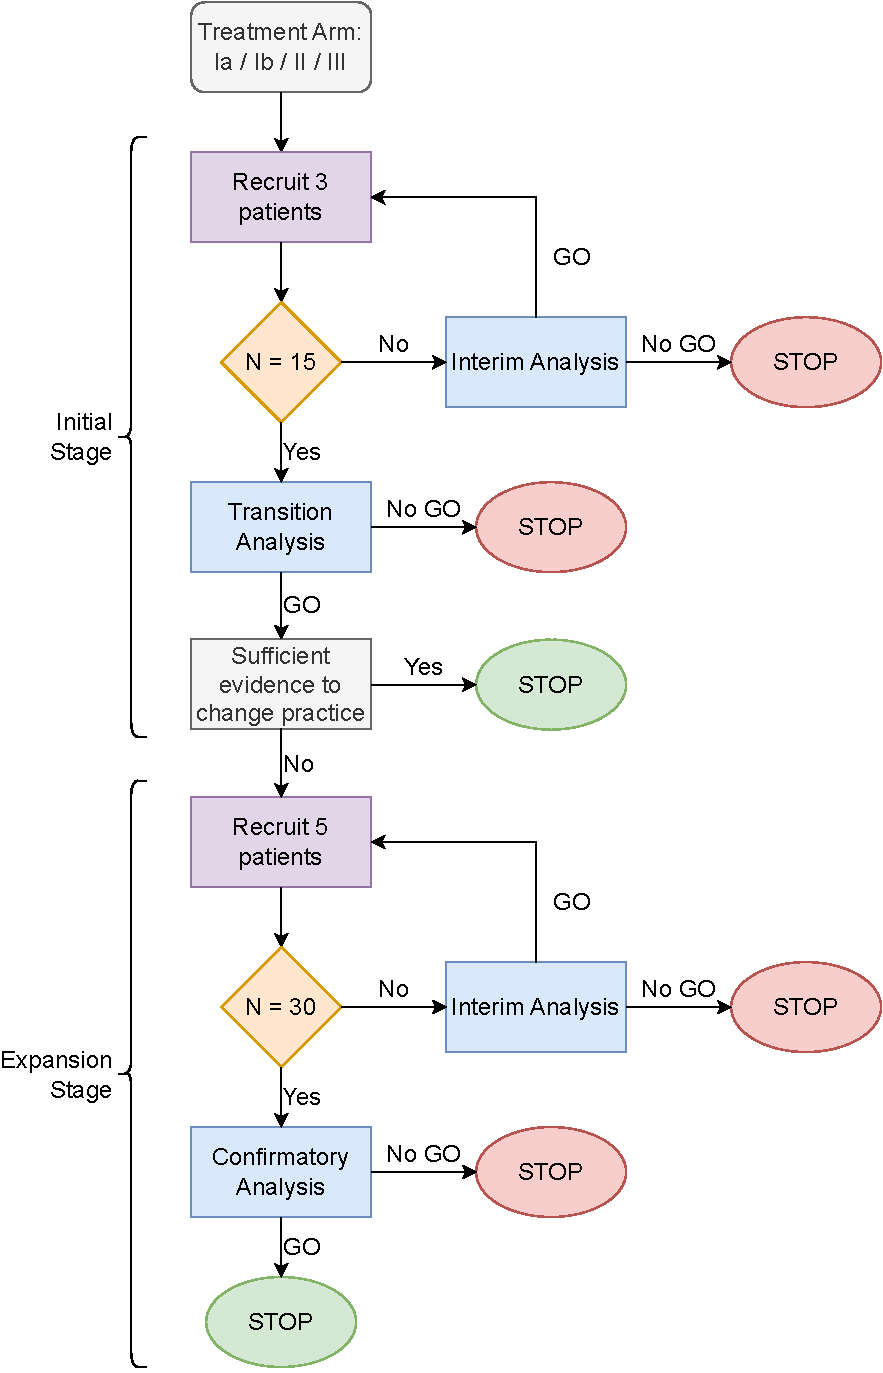
\includegraphics[width=0.9\textwidth]{ETP-GloBNHL-flowchart}
\end{figure}

A beta-binomial conjugate analysis will be conducted for each treatment arm. Observed trial data will be combined with a minimally informative Beta(1,1) prior to produce a posterior probability distribution for the treatment effect $\theta$, which represents either the OR/CR rate dependent on treatment arm. The posterior probability distribution is then used to inform decision making. GO/No Go decision criteria are specified separately for each treatment arm. 

For treatment arm \RN{1}a the decision criteria at the transition analysis is P($\theta$ > 40\%) $\geq$ 0.8. So, if the true OR rate was greater than 40\% with a probability of at least 0.8 based on the data collected in the trial there would be a GO decision. This corresponds to observing at least eight responses out of 15. For the confirmatory analysis a GO decision is made if P($\theta$ > 40\%) $\geq$ 0.95. At the final analysis we would need the probability that the true OR rate was greater than 40\% to be at least 0.95. Here a GO decision would only be made if 17 out of 30 patients had an OR. Table \ref{tab_etp:GloBNHL_decision_criteria} details the criteria for each treatment arm which can be interpreted in a similar manner. 

\begin{table}[h!]
	\centering
	\caption{Summary of decision criteria for Glo-BNHL.}
	\label{tab_etp:GloBNHL_decision_criteria}
	\resizebox{\textwidth}{!}{%
		\begin{tabular}{ccccc}
			\hline
			\multicolumn{1}{l}{\textbf{}} & \multicolumn{2}{c}{\textbf{Transition Analysis}}               & \multicolumn{2}{c}{\textbf{Confirmatory Analysis}}             \\ \cline{2-5} 
			\textbf{Treatment Arm}        & \textbf{Decision Criteria} & \textbf{Min No. Responses for GO} & \textbf{Decision Criteria} & \textbf{Min No. Responses for GO} \\ \hline
			Ia  & P($\theta$ \textgreater 40\%) $\geq$ 0.8 & 8/15 & P($\theta$ \textgreater 40\%) $\geq$ 0.95 & 17/30 \\
			Ib  & P($\theta$ \textgreater 10\%) $\geq$ 0.8 & 3/15 & P($\theta$ \textgreater 10\%) $\geq$ 0.95 & 6/30  \\
			II  & P($\theta$ \textgreater 20\%) $\geq$ 0.8 & 5/15 & P($\theta$ \textgreater 20\%) $\geq$ 0.95 & 10/30 \\
			III & P($\theta$ \textgreater 10\%) $\geq$ 0.8 & 3/15 & P($\theta$ \textgreater 10\%) $\geq$ 0.95 & 6/30  \\ \hline
		\end{tabular}%
	}
\end{table}

For the interim analyses there are separate stopping rules. These are the same across the treatment arms but differ in the initial stage compared to the expansion stage. During the initial stage, the predicted probability of success at the transition analysis (PPoSt) is calculated and decisions are made based on the following criteria: 

\begin{enumerate}
	\item PPoSt < 0.01 - recommend stopping for futility
	\item 0.01 $\leq$ PPoSt < 0.05 - consider stopping for futility
	\item 0.05 $\leq$ PPoSt < 0.15 - consider whether sufficient benefit in continuing 
	\item PPoSt $\geq$ 0.15 - recommend continuing 
\end{enumerate}

So, if the probability of success at the transition analysis is less than 1\% the recommendation would be to stop recruitment to the treatment arm and if it was greater than or equal to 15\% the recommendation would be to continue recruitment. If PPoSt is between 1-5\% or 5-15\% stopping should be also be considered for either futility or if there sufficient benefit in continuing respectively.  

At the expansion stage, the predicted probability of success at the confirmatory analysis is used (PPoSc). If this is below 10\% (PPoSc < 0.1) the recommendation would be to stop recruitment to that treatment arm due to futility. It should be noted that these decision rules are only recommendations and the independent data monitoring committee (DMC) will make decisions based on not only primary outcomes but secondary outcomes, recruitment and safety data. 

For this trial ETPs were produced separately for each treatment arm and for each stage. This resulted in eight ETPs, one for the initial stage showing the outcome of the transition analysis and one for the expansion stage showing the outcome of the confirmatory analysis for each treatment arm (\RN{1}a, \RN{1}b, \RN{2}, \RN{3}). ETPs were utilised throughout the design of the trial with initial versions originally created by GH using STATA and Microsoft PowerPoint. These were then further developed by SM who performed calculations in R but still utilised PowerPoint to create the ETPs. Figure \ref{fig_etp:GloBNHL-ETP-TA1aInitial} and \ref{fig_etp:GloBNHL-ETP-TA1aExtenstion} shows the ETPs for the initial and expansion stage of treatment arm \RN{1}a respectively. These ETPs created by SM helped us determine how our function and app visually presented ETPs and we utilised a similar colour scheme. 

Similar to MonoGerm the process of creating these ETPs in PowerPoint can be time consuming. This is even more of an issue in the Glo-BNHL study due to the multiple treatment arms and stages. Additionally, this trial highlighted another issue when you have multiple statisticians working on a trial who use different software packages. In this case it would mean work would have to be recreated in R and STATA to conduct the calculations required for ETPs. This served as further motivation for the development of an application which requires no specific stats software knowledge. As statisticians would easily be able to recreate ETPs. SM went on to further extend the function we developed to automatically generate ETPs specific to Glo-BNHL. 

\begin{sidewaysfigure}[h!]
	\centering
	\caption{ETP for the initial stage of treatment arm \RN{1}a in Glo-BNHL.}
	\label{fig_etp:GloBNHL-ETP-TA1aInitial}
	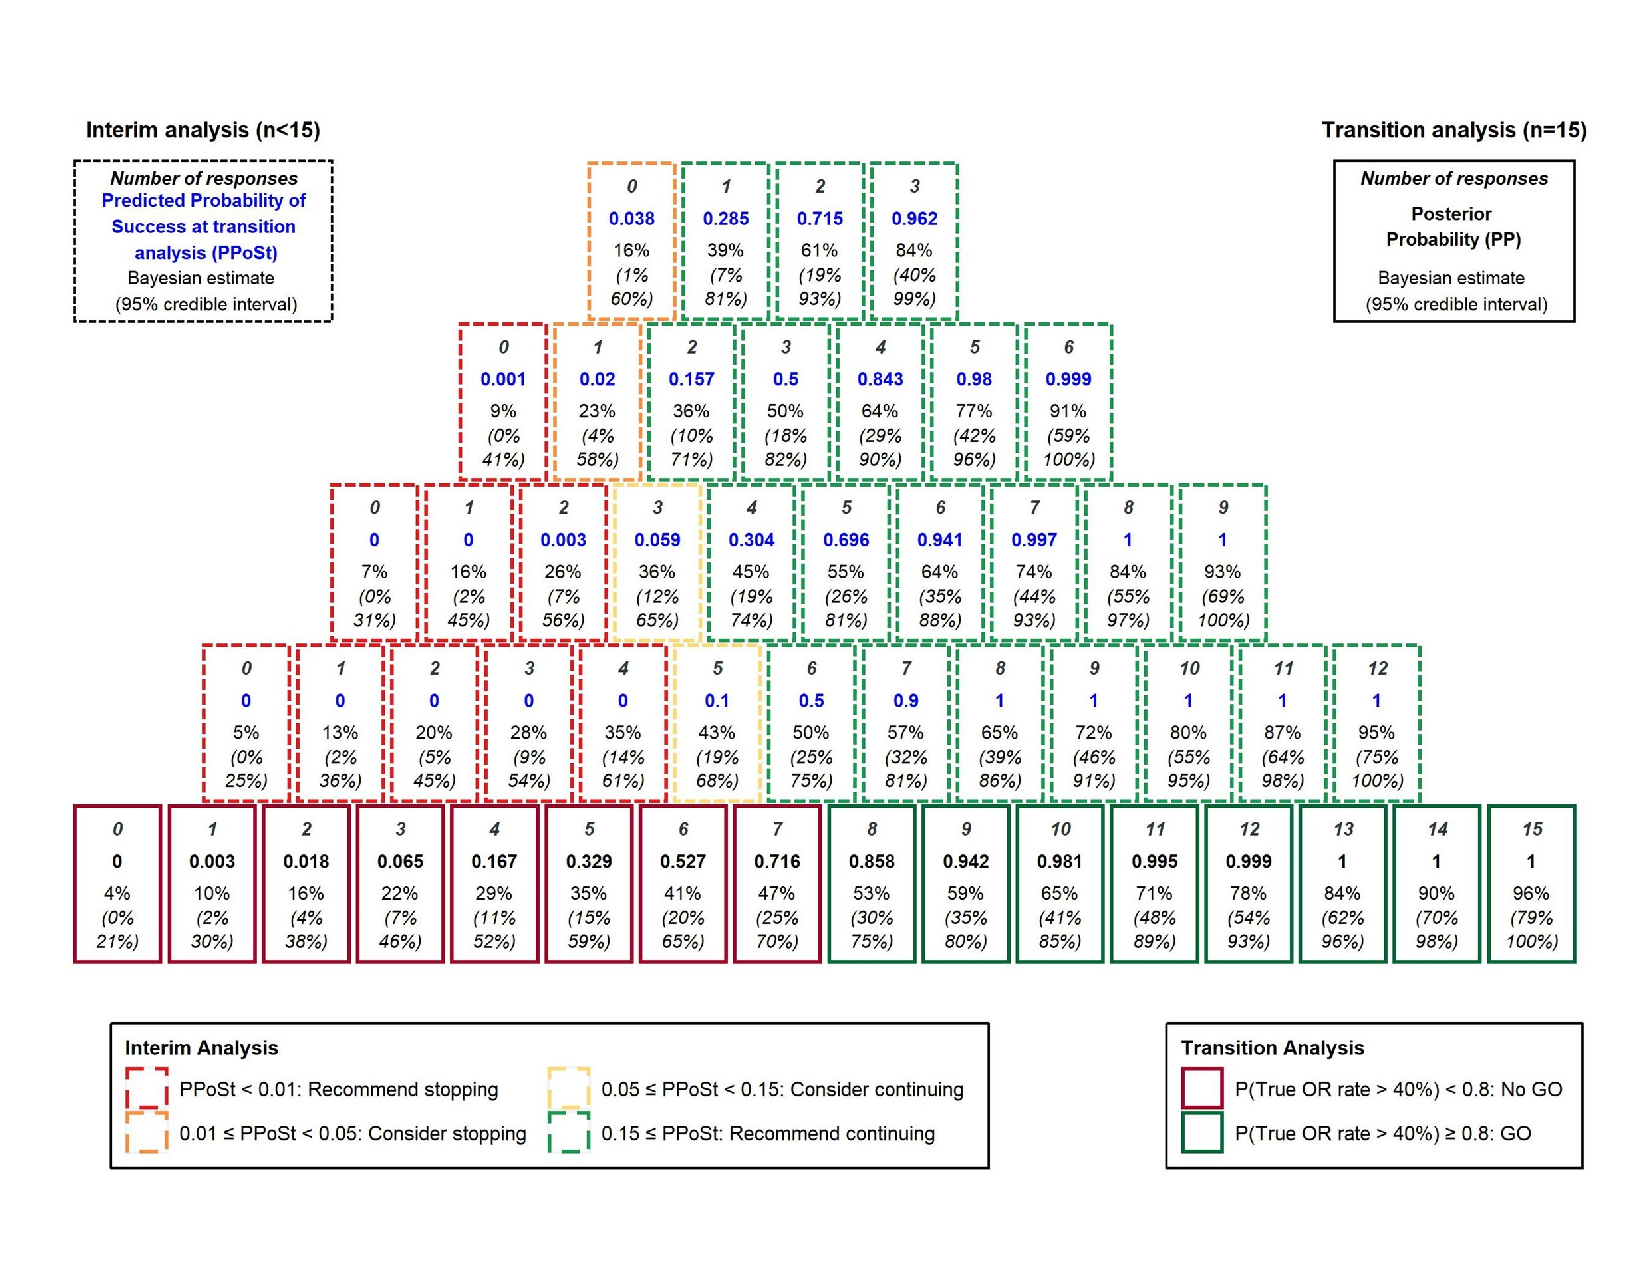
\includegraphics[width=23cm, height=15cm]{ETP-GloBNHL-ETP-TA1aInitial}
\end{sidewaysfigure} 

\begin{sidewaysfigure}[h!]
	\centering
	\caption{ETP for the expansion stage of treatment arm \RN{1}a in Glo-BNHL.}
	\label{fig_etp:GloBNHL-ETP-TA1aExtenstion}
	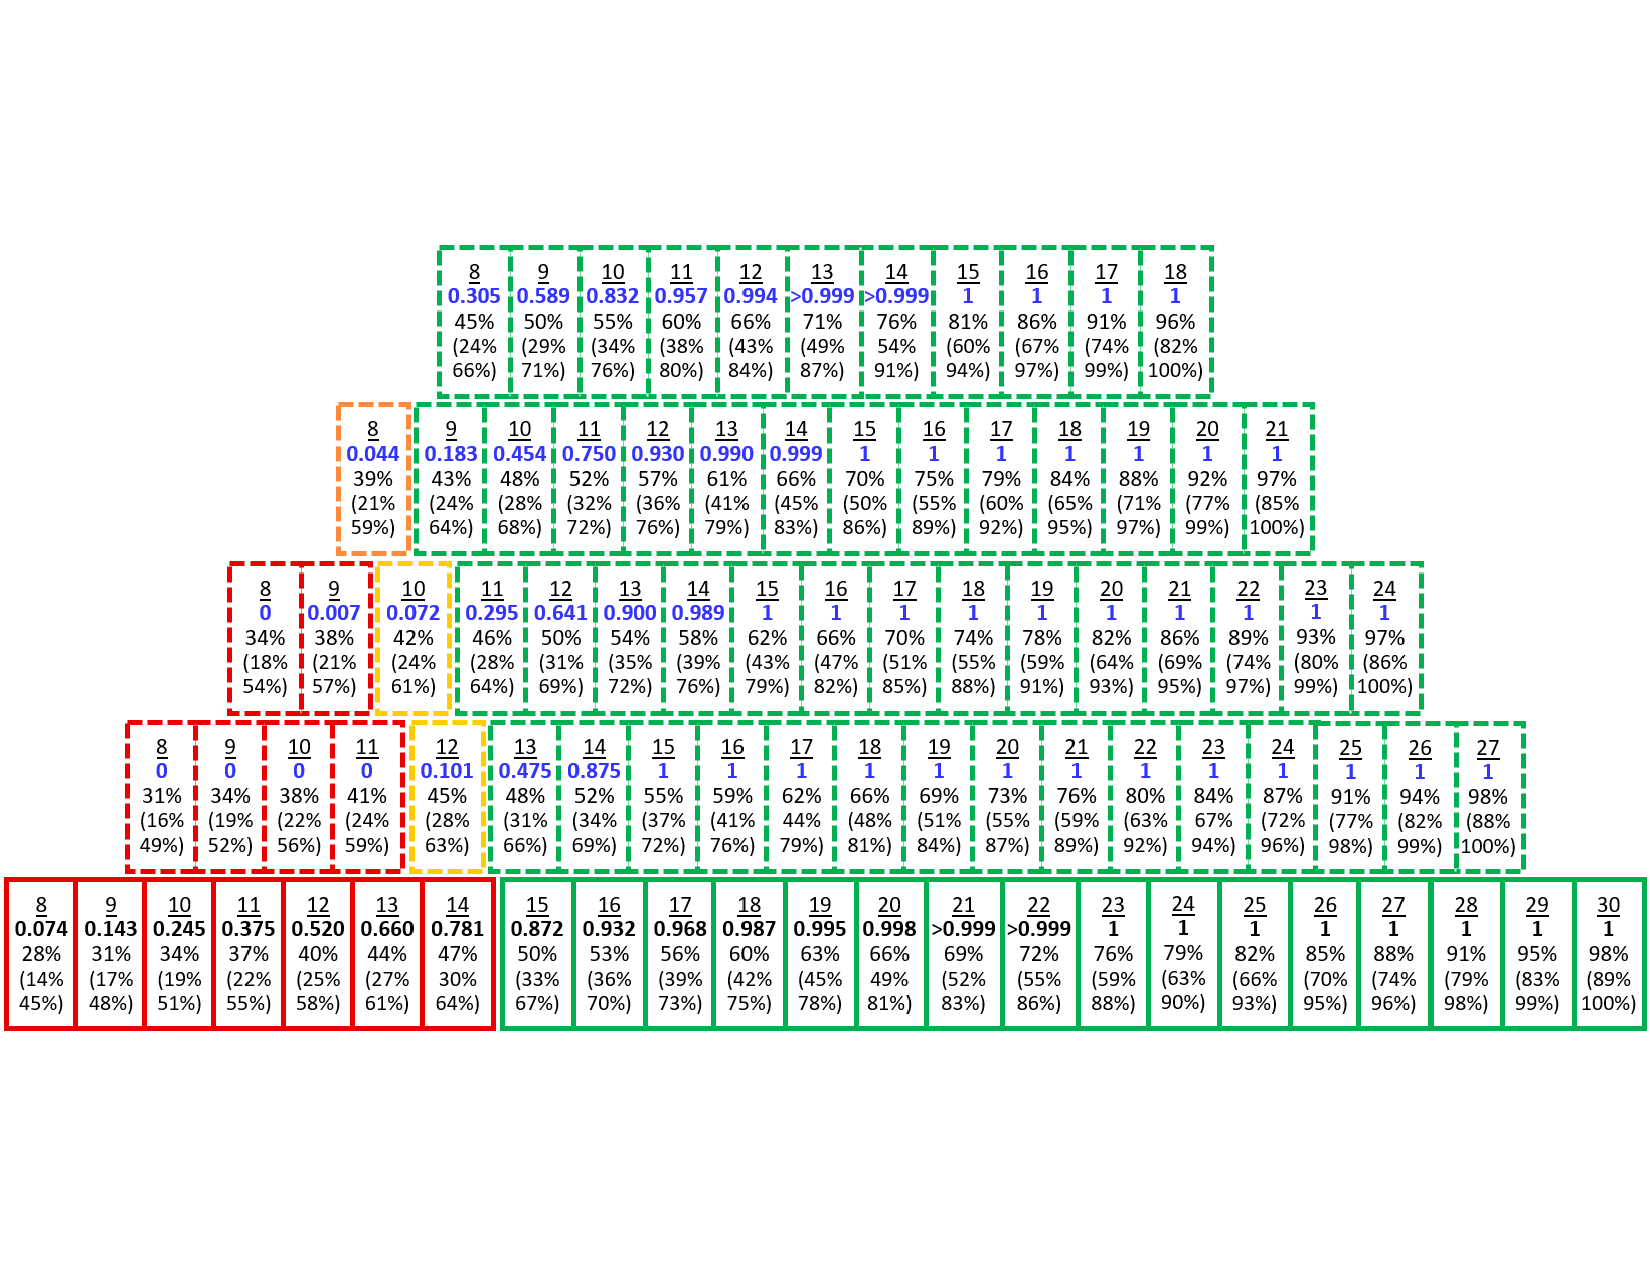
\includegraphics[width=23cm, height=15cm]{ETP-GloBNHL-ETP-TA1aExtension}
\end{sidewaysfigure} 

\clearpage

%-----------------------------------
%	SUBSECTION 3
%-----------------------------------

\section{DETERMINE}

DETERMINE \footnote{Determining Extended Therapeutic indications for Existing drugs in Rare Molecularly-defined Indications using a National Evaluation platform trial} is a trial that was also designed by Lucinda Billingham (LB). It is an umbrella-basket platform trial with multiple treatment arms running in parallel. The trial aims to evaluate the efficacy of targeted therapies in rare cancers with actionable genomic alterations, including common cancers with rare actionable alterations. This trial is currently open to recruitment and may be expanded in the future as more drugs are bought onto the platform.  

DETERMINE will recruit patients of all ages including, paediatric, TYA (teenage and young adult) and adults, who have rare tumours that contain an actionable genetic alteration that can be targeted therapeutically. The genetic alteration must have been identified previously from a tissue biopsy or ctDNA (circulating tumour DNA). Patients will then be stratified into molecular groups based on their tumour profile and allocated to the most suitable treatment arm by the Molecular Tumour Board (MTB). The umbrella part of the design consists of multiple non-randomised treatment arms, each evaluation a licensed targeted anti-cancer drug or drug combination in a specific molecularly-defined group of patients. Each molecularly-defined group allocated to a specific treatment arm will contain multiple baskets of different tumour types, age groups and molecular subtypes. This is visualised in Figure \ref{fig_etp:DETERMINEDesign}. 

\begin{figure}[h!]
	\centering
	\caption{Umbrella-basket platform trial design in DETERMINE.}
	\label{fig_etp:DETERMINEDesign}
	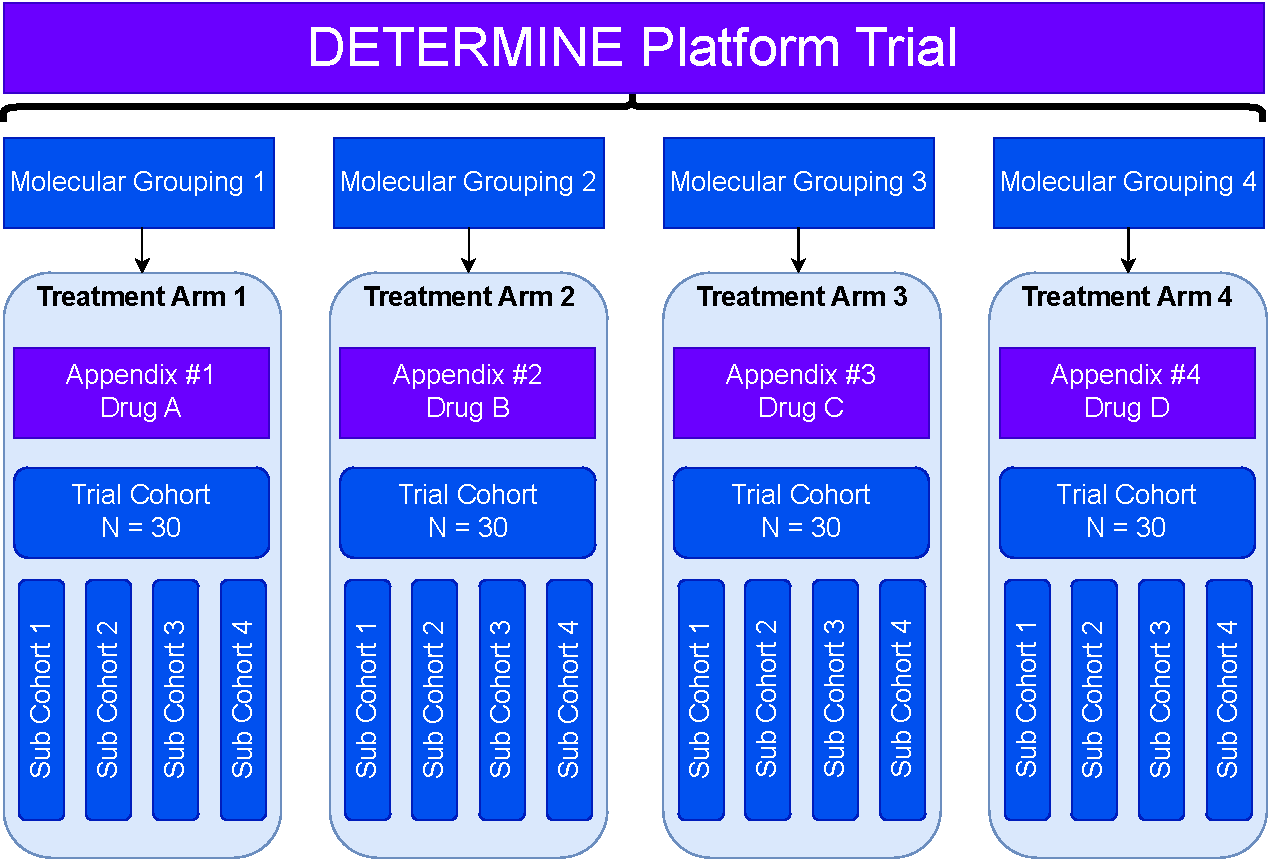
\includegraphics[width=\textwidth]{ETP-DETERMINEDesign}
\end{figure}

A main trial cohort of 30 evaluable patients will be recruited into each treatment arm. This will include patients with different tumour types, ages and molecular subtypes. If specific subgroups within this main cohort are experiencing significant benefit from treatment sub-cohorts will be formed to investigate treatment effectiveness in these subgroups. It is possible for each treatment arm to have multiple sub-cohorts and they can recruit in parallel to the main cohort. Each sub-cohort will be subject to the same statistical analysis and will also aim to recruit 30 patients. Currently there are five treatment arms, details of these are provided in Table \ref{tab_etp:DETERMINE_trtarms}. 

\begin{table}[h!]
	\fontsize{10pt}{10pt}\selectfont
	\centering
	\caption{Current treatment arms in DETERMINE}
	\label{tab_etp:DETERMINE_trtarms}
	\resizebox{\textwidth}{!}{%
		\begin{tabular}{p{0.1\textwidth} | p{0.2\textwidth} | p{0.5\textwidth} | p{0.2\textwidth}}
			Treatment Arm  & IMP(s) & Molecular Grouping & Route and Formulation \\ \hline
			1 &  Alectinib & ALK gene fusion positive solid tumours & Oral capsules \\ \hline
			2 & Atezolizumab & Solid tumours with high tumour mutational burden (TMB) or microsatellite instability-high (MSI-high) or proven constitutional mismatch repair deficiency (CMMRD) disposition & Intravenous (IV) infusion  \\ \hline
			3 & Entrectinib & NTRK or ROS1 gene fusion positive solid tumours & Oral capsules; Dosing depends on body surface area (BSA) \\ \hline
			4 & Trastuzumab in combination with pertuzumab & Solid tumours with HER2 amplification or mutations & IV infusion \\ \hline 
			5 & Vemurafenib in combination with cobimetinib & Solid tumours with BRAF V600 mutations & Oral; 960 mg tablets \\ \hline
		\end{tabular}
	}
\end{table}

Co-primary outcomes of objective response (OR) and durable clinical benefit (DCB) will be used to assess efficacy of the treatment in each of the cohorts in each molecular grouping. These are both classified as binary variables. OR is defined dependent on specific disease criteria. DCB is defined as the absence of disease progression for at least 24 weeks from the start of trial treatment, this will also be measured based on disease specific criteria. Patients will receive treatment based on the license schedule for the drug in their treatment arm. Patients continue treatment until either they reach progressive disease (PD), unacceptable adverse events or withdraw from the trial. 

All outcomes in each treatment arm, cohort and sub cohort will be analysed using a Beta-Binomial conjugate analysis. Posterior probability distributions for OR and DCB will be generated using minimally informative priors, Beta(0.1,0.9) and data that is collected on the trial. However decision making will be done using the BOP-2 design \cite{zhouBOP2BayesianOptimal2017,zhouBayesianOptimalPhase2020}. This design makes GO or No GO decisions by assessing posterior probabilities for a set of outcomes, which are optimised to either maximise power or minimise the number of patients. The design also allows for the control of type I and type II error rates. In DETERMINE, for each co-primary outcome, a rate of 10\% or less would represent a treatment effect that is not clinically relevant and a rate of 30\% would represent a clinically meaningful treatment effect. These can be thought of as a null and alternative hypothesis. The use of this design was made possible due to the development of web applications by the authors at the MD Anderson Cancer Centre \cite{tidwellBayesianClinicalTrials2019}. 

Interim analyses will be conducted throughout the trial, however formal decision making will first be conducted after 10 evaluable patients have been recruited and then every 5 patients from that time-point in each cohort/sub-cohort. If probability that both the true OR and DCB rates are lower than the critical threshold of 10\% the trial would recommend stopping. The design is optimised to minimise the type II error i.e. to minimise the probability of not rejecting the null hypothesis when treatment is effective. This is done whilst controlling the type I error rate at 0.1. Under the BOP-2 design this provides the following stopping boundaries of 0/10, $\leq$1/15, $\leq$2/20, $\leq$3/25 at each of the planned analyses at 10, 15, 20 and 25 patients. For the final analysis at 30 patients there would be a GO decision if $\geq$6/30 patients had either a OR or DCB.   

The ETPs we have shown so far all have been based on a Beta-Binomial conjugate analysis with decisions made using PPoS and the posterior distribution. However, they can also be utilised here. LB created the ETP shown in Figure \ref{fig_etp:DETERMINE-ETP}. Here we can see each cell still pertains to a specific number of responses out of a certain number of patients. Bayesian estimates, credible intervals and posterior probabilities of the treatment effect being greater than our null and alternative hypothesis. The cells have then been colour coded based on the decision criteria elicited from the BOP-2 design. This trial also shows that ETPs are a flexible tool that can also be applied to trials not explicitly using a Beta-Binomial conjugate analysis for decision making. 

\begin{sidewaysfigure}[h!]
	\centering
	\caption{ETP for the DETERMINE trial.}
	\label{fig_etp:DETERMINE-ETP}
	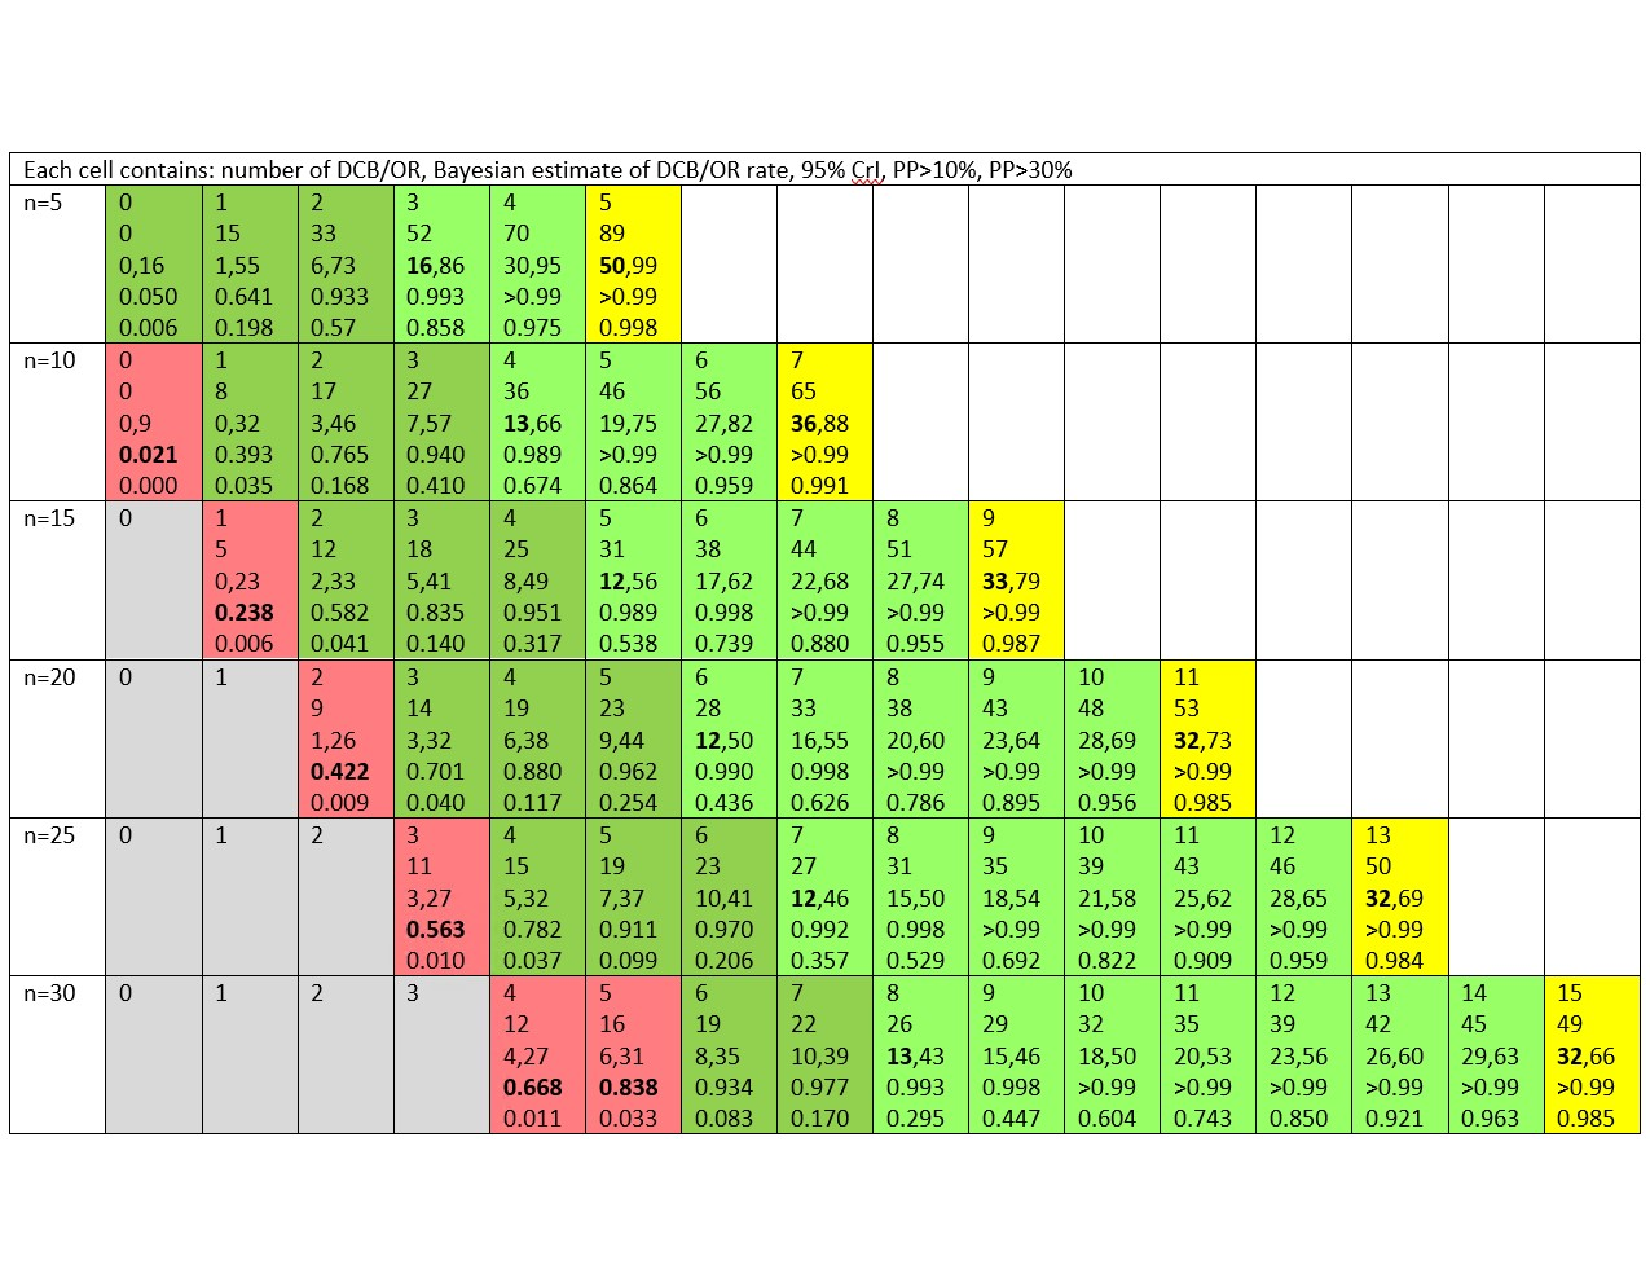
\includegraphics[width=23cm, height=15cm]{ETP-DETERMINE-ETP}
\end{sidewaysfigure} 

\clearpage